\documentclass{beamer}

\usetheme{simple}

\usepackage{caption}
\usepackage{xcolor}
\usepackage{fancyvrb}
\usepackage{ulem}
\usepackage{subcaption}
\usetikzlibrary{positioning,calc,automata}

\title{CSC363 Tutorial \#7}
\subtitle{\textit{Alternative} TMs}
\date{March 9, 2022}
\institute{}

\newcommand{\N}{{\mathbb N}}
\newcommand{\R}{{\mathbb R}}
\newcommand{\inner}[1]{\langle #1 \rangle}

\setwatermark{\includegraphics[height=8cm]{img/chungus.png}}

\begin{document}

\maketitle

\begin{frame}{Learning objectives this tutorial}
\begin{itemize}
\item Define some aliases we'll be using for this part of the course (complexity).
\item Describe a ``multi-tape'' TM.
\item Show that a multi-tape TM is effectively just a TM, but slightly better.
\end{itemize}
\end{frame}

\begin{frame}{Some aliases}

In the \textit{computability} part of the course, we've discussed the ``solvability'' of \textit{sets} (all subsets of our universe $\N$).

\vspace{2mm} \pause

In the \textit{complexity} part of the course, our universe is $\Sigma^*$ (the set of strings using characters from $\Sigma$) instead of $\N$, where $\Sigma$ is some predetermined alphabet (binary, decimals, ASCII characters, and others).

\vspace{2mm} \pause

\textbf{Task:} Let $\Sigma$ be any finite alphabet. There is a natural correspondence between $\Sigma^*$ and $\N$, as we can assign each string a \textit{unique} natural number. Recall what we used to show this.

\vspace{2mm} \pause

\textbf{Ans:} G\"odel Numbers!

$$\text g \rightarrow 7, \text o \rightarrow 15, \text d \rightarrow 4, \text e \rightarrow 5, \text l \rightarrow 12$$
$$\text{godel} \rightarrow 2^7 3^{15} 5^{4} 7^{5} 11^{12}$$

\end{frame}

\begin{frame}{Some aliases}
\textbf{Task:} Let $\Sigma$ be any finite alphabet. There is a natural correspondence between $\Sigma^*$ and $\N$, as we can assign each string a \textit{unique} natural number. Recall what we used to show this.

\vspace{2mm} \pause

\textbf{Ans:} G\"odel Numbers!

$$\text g \rightarrow 7, \text o \rightarrow 15, \text d \rightarrow 4, \text e \rightarrow 5, \text l \rightarrow 12$$
$$\text{godel} \rightarrow 2^7 3^{15} 5^{4} 7^{5} 11^{12}$$

\vspace{4mm}

So in this sense, subsets of $\Sigma^*$ can be thought of as subsets of $\N$ by mapping $S \subseteq \Sigma^*$ to $g(S) = \{g(w): w \in S\} \subseteq \N$, where $g$ is the G\"odel mapping function.

\vspace{2mm} \pause

\textbf{Question:} What is another term for a subset of $\Sigma^*$?

\pause

\textbf{Ans:} \textit{Language}.

\vspace{2mm}


\end{frame}

\begin{frame}{Some aliases}

In complexity, we will consider the efficient \textit{decidability} of languages.

\vspace{2mm}

\textbf{Question:} What is another word for \textit{decidable}?

\pause

\textbf{Ans:} \textit{Computable}.

\vspace{2mm}

Most languages we consider in complexity theory are decidable; we examine whether they are decidable \textit{efficiently}.

\vspace{2mm} \pause

\textbf{Definition:} A \textit{decider} for a language $L$ is a TM that: 
\begin{enumerate}
    \item always halts \textit{on any input},
    \item accepts the input $x$ if and only if $x \in L$.
\end{enumerate}

\end{frame}


\begin{frame}{Multi-tape TM}

\textbf{Task:} Describe some attributes we could add to a TM to make it ``multi-tape''. What will the transition function look like? How is input handled?

\vspace{2mm} \pause

Here's what I have in mind:

\begin{center}
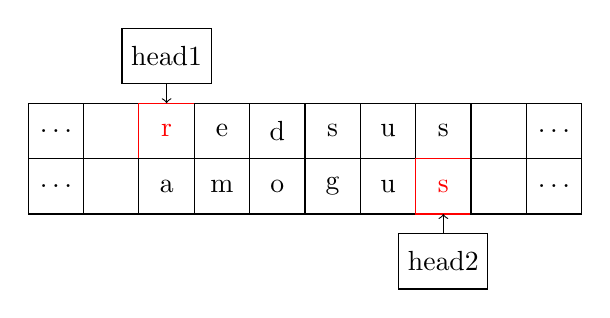
\begin{tikzpicture}[every node/.style={block},
        block/.style={minimum height=2em,minimum width=2em,outer sep=0pt,draw,rectangle,node distance=0pt}]
   \node (R1) {$\ldots$};
   \node (R2) [right=of R1] {$\square$};
   \node (R3) [right=of R2, color=red] {r};
   \node (R4) [right=of R3] {e};
   \node (R5) [right=of R4] {d};
   \node (R6) [right=of R5] {s};
   \node (R7) [right=of R6] {u};
   \node (R8) [right=of R7] {s};
   \node (R10) [right=of R8] {$\square$};
   \node (R11) [right=of R10] {$\ldots$};
   \node (R12) [below=of R1] {$\ldots$};
   \node (R13) [right=of R12] {$\square$};
   \node (R14) [right=of R13] {a};
   \node (R15) [right=of R14] {m};
   \node (R16) [right=of R15] {o};
   \node (R17) [right=of R16] {g};
   \node (R18) [right=of R17] {u};
   \node (R19) [right=of R18, color=red] {s};
   \node (R21) [right=of R19] {$\square$};
   \node (R22) [right=of R21] {$\ldots$};
   \node (HEAD1) [above = 0.25cm of R3] {head1};
   \draw[->] (HEAD1) -- (R3);
   \node (HEAD2) [below = 0.25cm of R19] {head2};
   \draw[->] (HEAD2) -- (R19);
\end{tikzpicture}
\end{center}

\end{frame}


\begin{frame}{Multi-tape TM}
\textbf{Definition:} A \textbf{$k$-tape Turing Machine} is like an ordinary Turing Machine, but its transition function is now
$$\delta: Q \times \Gamma^k \to Q \times \Gamma^k \times \{L, R\}^k.$$
In effect, this gives us $k$ distinct tapes, each with its own read/write head. We read and write $k$ symbols at once. \pause

\vspace{2mm}

The input is placed on the first tape; all other tapes start blank. 
\end{frame}

\begin{frame}{Multi-tape TM Example}

Let's construct a multi-tape TM over the alphabet $\{0, 1\}$ that accepts palindromes. Here's what we will do:

\begin{center}
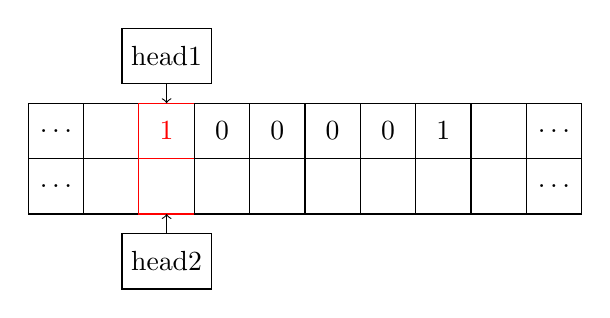
\begin{tikzpicture}[every node/.style={block},
        block/.style={minimum height=2em,minimum width=2em,outer sep=0pt,draw,rectangle,node distance=0pt}]
   \node (R1) {$\ldots$};
   \node (R2) [right=of R1] {$\square$};
   \node (R3) [right=of R2, color=red] {1};
   \node (R4) [right=of R3] {0};
   \node (R5) [right=of R4] {0};
   \node (R6) [right=of R5] {0};
   \node (R7) [right=of R6] {0};
   \node (R8) [right=of R7] {1};
   \node (R10) [right=of R8] {$\square$};
   \node (R11) [right=of R10] {$\ldots$};
   \node (R12) [below=of R1] {$\ldots$};
   \node (R13) [right=of R12] {$\square$};
   \node (R14) [right=of R13, color=red] {$\square$};
   \node (R15) [right=of R14] {$\square$};
   \node (R16) [right=of R15] {$\square$};
   \node (R17) [right=of R16] {$\square$};
   \node (R18) [right=of R17] {$\square$};
   \node (R19) [right=of R18] {$\square$};
   \node (R21) [right=of R19] {$\square$};
   \node (R22) [right=of R21] {$\ldots$};
   \node (HEAD1) [above = 0.25cm of R3] {head1};
   \draw[->] (HEAD1) -- (R3);
   \node (HEAD2) [below = 0.25cm of R14] {head2};
   \draw[->] (HEAD2) -- (R14);
\end{tikzpicture}
\end{center}

\begin{enumerate}
    \item Copy the string on tape 1 to tape 2.
    \item Move head1 to the beginning of the first tape. 
    \item Compare characters from head1 and head2, scanning right and left respectively.
\end{enumerate}

\end{frame}

\begin{frame}{Multi-tape TM Example}

\begin{center}

\begin{enumerate}
    \item Copy the string on tape 1 to tape 2.
\end{enumerate}

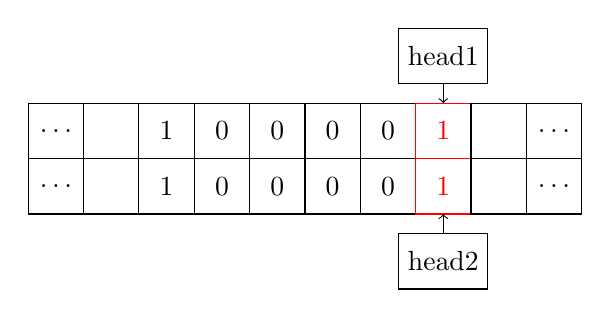
\begin{tikzpicture}[every node/.style={block},
        block/.style={minimum height=2em,minimum width=2em,outer sep=0pt,draw,rectangle,node distance=0pt}]
   \node (R1) {$\ldots$};
   \node (R2) [right=of R1] {$\square$};
   \node (R3) [right=of R2] {1};
   \node (R4) [right=of R3] {0};
   \node (R5) [right=of R4] {0};
   \node (R6) [right=of R5] {0};
   \node (R7) [right=of R6] {0};
   \node (R8) [right=of R7, color=red] {1};
   \node (R10) [right=of R8] {$\square$};
   \node (R11) [right=of R10] {$\ldots$};
   \node (R12) [below=of R1] {$\ldots$};
   \node (R13) [right=of R12] {$\square$};
   \node (R14) [right=of R13] {1};
   \node (R15) [right=of R14] {0};
   \node (R16) [right=of R15] {0};
   \node (R17) [right=of R16] {0};
   \node (R18) [right=of R17] {0};
   \node (R19) [right=of R18, color=red] {1};
   \node (R21) [right=of R19] {$\square$};
   \node (R22) [right=of R21] {$\ldots$};
   \node (HEAD1) [above = 0.25cm of R8] {head1};
   \draw[->] (HEAD1) -- (R8);
   \node (HEAD2) [below = 0.25cm of R19] {head2};
   \draw[->] (HEAD2) -- (R19);
\end{tikzpicture}
\end{center}

\end{frame}

\begin{frame}{Multi-tape TM Example}

\begin{center}

\begin{enumerate}
    \setcounter{enumi}{2}
    \item Compare characters from head1 and head2, scanning right and left respectively.
\end{enumerate}

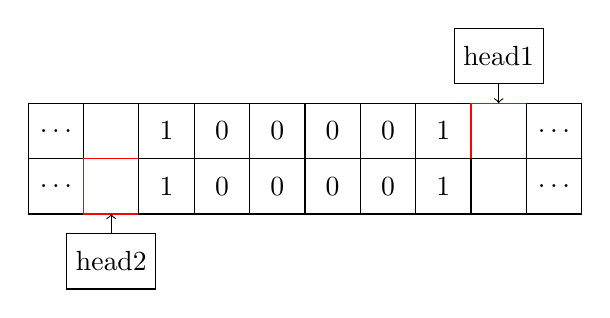
\begin{tikzpicture}[every node/.style={block},
        block/.style={minimum height=2em,minimum width=2em,outer sep=0pt,draw,rectangle,node distance=0pt}]
   \node (R1) {$\ldots$};
   \node (R2) [right=of R1] {$\square$};
   \node (R3) [right=of R2] {1};
   \node (R4) [right=of R3] {0};
   \node (R5) [right=of R4] {0};
   \node (R6) [right=of R5] {0};
   \node (R7) [right=of R6] {0};
   \node (R8) [right=of R7] {1};
   \node (R10) [right=of R8, color=red] {$\square$};
   \node (R11) [right=of R10] {$\ldots$};
   \node (R12) [below=of R1] {$\ldots$};
   \node (R13) [right=of R12, color=red] {$\square$};
   \node (R14) [right=of R13] {1};
   \node (R15) [right=of R14] {0};
   \node (R16) [right=of R15] {0};
   \node (R17) [right=of R16] {0};
   \node (R18) [right=of R17] {0};
   \node (R19) [right=of R18] {1};
   \node (R21) [right=of R19] {$\square$};
   \node (R22) [right=of R21] {$\ldots$};
   \node (HEAD1) [above = 0.25cm of R10] {head1};
   \draw[->] (HEAD1) -- (R10);
   \node (HEAD2) [below = 0.25cm of R13] {head2};
   \draw[->] (HEAD2) -- (R13);
\end{tikzpicture}
\end{center}
\end{frame}

\begin{frame}{Multi-tape TM Example}

\textbf{Question:} What runtime (in terms of length of input $n$) does this $2$-tape TM have?

\pause

\textbf{Ans:} $O(n)$ (because we have to keep jumping back and forth).

\vspace{2mm} \pause

\textbf{Question:} What runtime (in terms of length of input $n$) would a ``naive'' single-tape TM use to detect palindromes?

\pause

\textbf{Ans:} $O(n^2)$ (because we have to keep jumping back and forth).

\end{frame}

\begin{frame}{Multi-tape TM Example}

\textbf{Task:} Construct a $O(n)$ $2$-tape TM that decides the language $\{0^n 1^n: k \in \N\}$. You may use a high-level description if you want.

\pause

\textbf{Ans:} Here's the procedure I have in mind.

\begin{enumerate}
    \item Copy the string on tape 1 to tape 2.
    \item Move head1 to the beginning of the first tape. 
    \item Compare character by character; if head1 and head2 both read $0$ or both read $1$, then reject.
\end{enumerate}

\end{frame}

\begin{frame}{Multi-tape TM Example}
\textbf{Question:} How fast can we decide $\{0^n 1^n: k \in \N\}$ with a TM?

\pause

\textbf{Ans:} Naively, $O(n^2)$. The procedure is as follows:
\begin{enumerate}
    \item Cross out a $0$; move to the right end of the string.
    \item Cross out a $1$; move to the left end of the string.
\end{enumerate}
Try \url{https://turingmachinesimulator.com/shared/prsswhkkyb}.

\vspace{2mm} \pause

But we can do better! There is a $O(n \log n)$ procedure:

\pause

\begin{enumerate}
    \item Scan across the tape and reject if a $0$ is found to the right of a $1$.
    \item Repeat the following as long as there is both a $0$ and a $1$ on the tape:
    \begin{enumerate}
        \item Scan across the tape, and reject if the total number of $0$s and $1$s remaining is odd.
        \item Scan again across the tape, crossing off every other $0$, and crossing off every other $1$.
    \end{enumerate}
    \item If the tape doesn't have any $0$s or $1$s, accept. Else, reject.
\end{enumerate}

\pause

Try \url{https://turingmachinesimulator.com/shared/bkuepwxgdh}.

\end{frame}


\begin{frame}{Multi-tape TMs in P}

It turns out, just as with NTMs, the question of \textit{decidability} doesn't change with multi-tape TMs.
\pause
\begin{itemize}
    \item Everything that is decidable with a NTM is also decidable with a TM (since we can simulate a NTM on a TM).
    \item Everything that is decidable with a $k$-tape TM is also decidable with a TM.
\end{itemize}

\pause

In fact, there is an even stronger theorem.\\

\textbf{Theorem:} Everything that is decidable with a $k$-tape TM in $O(f(n))$ time is decidable with a TM in $O((f(n))^2)$ time. (See Sipser page 137)

\vspace{2mm} \pause

\textbf{Task:} Using the above, show that any language that is poly-time decidable by a $k$-tape TM is also poly-time decidable by a TM.

\pause

\textbf{Ans:} If a language is decidable by a $O(n^p)$ $k$-tape TM, then according to the theorem, it is decidable by a $O(n^{2p})$ TM.

\vspace{2mm} \pause

In effect, this shows that multi-tape TMs are ``better'', but don't fundamentally change the set of poly-time decidable languages.


\end{frame}



\end{document}